\documentclass[11pt]{article}

\usepackage[margin=0.6in]{geometry}
\usepackage[T1]{fontenc}
\usepackage[utf8]{inputenc}
\usepackage{lmodern}
\usepackage{array}
\usepackage{booktabs}
\usepackage{enumitem}
\usepackage{float}
\usepackage{graphicx}
\usepackage{hyperref}
\usepackage{longtable}
\usepackage{natbib}
\usepackage{parskip}
\usepackage{ragged2e}
\usepackage{setspace}
\usepackage{tabularx}
\usepackage{titlesec}
\usepackage[table]{xcolor}
\usepackage{tikz}
\usepackage{wrapfig}

\usetikzlibrary{arrows.meta,positioning,shapes.geometric,fit,backgrounds}

\definecolor{PrimaryRed}{HTML}{8B1E1E}
\definecolor{SoftBlue}{HTML}{DDEEFF}
\definecolor{DarkGray}{HTML}{333333}
\definecolor{JoySoft}{HTML}{FFF8E8}

\hypersetup{colorlinks=true,linkcolor=black,urlcolor=black,citecolor=black}
\setlength{\parindent}{0pt}
\newcolumntype{Y}{>{\raggedright\arraybackslash}X}
\titleformat{\section}{\large\bfseries\color{PrimaryRed}}{}{0em}{}
\titleformat{\subsection}{\normalsize\bfseries\color{DarkGray}}{\thesubsection}{0.5em}{}
\setstretch{1.12}
\setlist[itemize]{topsep=1pt,itemsep=0pt,parsep=0pt,partopsep=0pt}
\setlist[enumerate]{topsep=1pt,itemsep=0pt,parsep=0pt,partopsep=0pt}

\begin{document}

\begin{titlepage}
\newgeometry{margin=0.95in}
\thispagestyle{empty}

\begin{center}
{\large University of Rochester\\}
{\normalsize Warner School of Education\\[0.35in]}

{\color{PrimaryRed}\rule{\textwidth}{1.4pt}}\\[0.22in]
{\Huge\bfseries Literacy as Power:\\[0.08in] Communication Access,\\[0.08in] Neurodivergence, and Social Justice\\[0.08in] in STEM Education}\\[0.18in]
{\Large Critical Literacy Journal}\\[0.22in]
{\color{PrimaryRed}\rule{0.78\textwidth}{0.7pt}}\\[0.32in]

\colorbox{SoftBlue}{%
\parbox{0.88\textwidth}{%
\centering\vspace{0.12in}
\textit{Communication Access as Literacy, Power, and Educational Justice}\\[0.05in]
A literacy and social justice analysis of classroom communication, disciplinary language, accommodation systems, and institutional literacy.
\vspace{0.12in}
}%
}
\end{center}

\vspace{0.25in}

\begin{center}
\renewcommand{\arraystretch}{1.15}
\setlength{\tabcolsep}{4pt}
\begin{tabular}{>{\bfseries\RaggedLeft}p{1.65in} p{4.9in}}
Student & Piter Zacari Garcia Bautista \\
Course & EDU498: Literacy Learning as Social Practice \\
Assignment & Literacy as Power: Bridging Social Justice and Critical Communication \\
Focus & Communication access injustice for neurodivergent and chronically ill students in STEM education \\
Present-Day Connection & Universal Design for Learning / CAST UDL Guidelines 3.0 \\
Submission Date & June 2026 \\
\end{tabular}
\end{center}

\vspace{0.25in}

\begin{center}
\begin{minipage}{0.95\textwidth}
\itshape
This journal uses a BIO/STEM communication access case as an evidence site for a broader literacy and social justice argument. It examines how classroom communication, disciplinary terminology, accommodation systems, and institutional pathways can determine whether students are understood, supported, and allowed to participate with dignity.
\end{minipage}
\end{center}

\restoregeometry
\end{titlepage}
\clearpage
\onehalfspacing

%% ─────────────────────────────────────────────
\section*{The Bridge}
%% ─────────────────────────────────────────────

\begin{wrapfigure}{r}{0.43\textwidth}
    \vspace{-4em}
    \centering
    
\includegraphics[
        width=0.43\textwidth,
        height=0.43\textheight,
        keepaspectratio
    ]{images/real_pain_real_injustice.png}
    {\scriptsize\textit{Figure 1. A visual map of communication harm, institutional rigidity, and the emotional burden created by inaccessible teaching design.}\par}
    \vspace{-1.5em}
\end{wrapfigure}

In this paper, literacy is not limited to reading and writing. In a STEM course, literacy also means decoding requirements, navigating accommodation systems, interpreting grading language, understanding unstated expectations, and finding one's way through institutional pathways. When a teacher designs communication around a single assumed learner, one who processes oral directions reliably, tolerates ambiguity, performs knowledge in approved formats, and advocates from a position of institutional fluency, they may unintentionally exclude neurodivergent, chronically ill, disabled, multilingual, trauma-impacted, and otherwise vulnerable students. This exclusion does not require malice; it requires only a narrow design. This paper uses a documented BIO/STEM communication access case as the primary evidence site for a larger social justice argument. The guiding question is pointed: if an adult graduate student with technical knowledge, documentation habits, advisor support, and self-advocacy experience can still be measurably harmed by inaccessible course communication, \textit{what happens to children who cannot yet name, document, or resist that harm?}

%% ─────────────────────────────────────────────
\section*{Communication Access as a Social Justice Issue}
%% ─────────────────────────────────────────────

\begin{wrapfigure}{l}{0.5\textwidth}
\vspace{-1.5em}
\centering
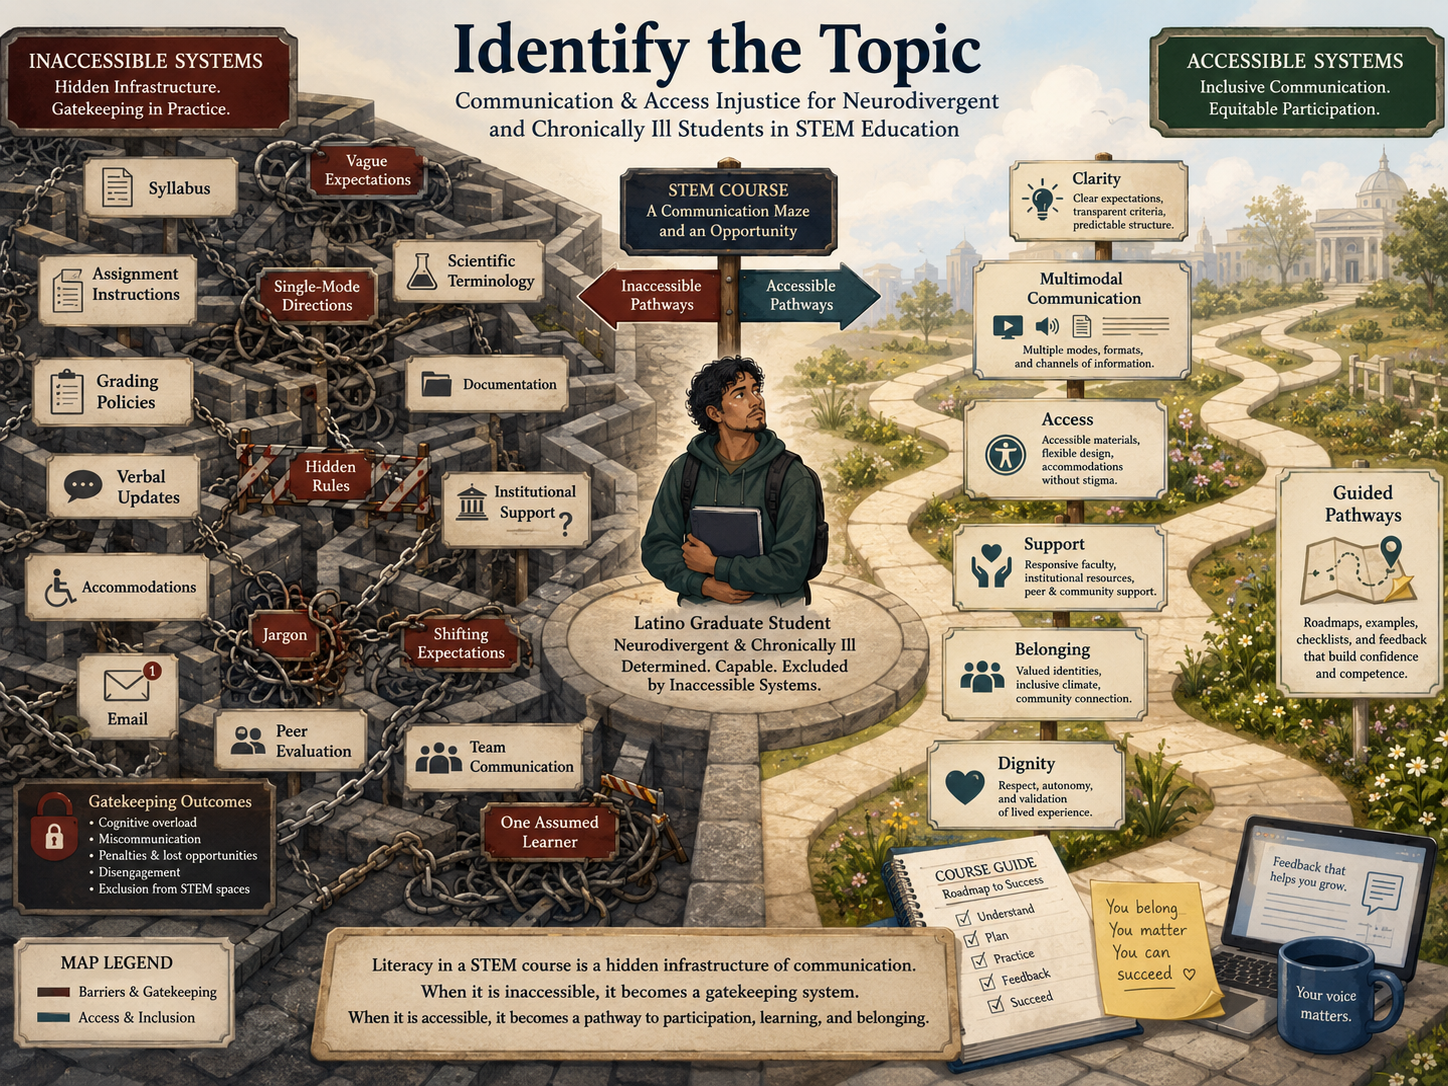
\includegraphics[
width=0.5\textwidth,
height=0.5\textheight,
keepaspectratio
]{images/identifying_the_real_topic.png}
{\scriptsize\textit{Figure 2. How communication breakdowns and institutional rigidity shift learning barriers from the system onto individual students.}\par}
\vspace{-1.2em}
\end{wrapfigure}

Communication access is a social justice issue because literacy in educational settings extends far beyond text. In a STEM course, students must simultaneously learn disciplinary content and navigate the communication systems that govern participation: the syllabus, assignment instructions, grading policies, accommodation procedures, team expectations, scientific conventions, verbal updates, and institutional escalation pathways. When those systems are clear, stable, multimodal, and teachable, they empower students to understand expectations, use available support, and demonstrate what they know. When those systems are vague, single-mode, memory-dependent, or designed around a narrow prototype of the successful learner, they function as barriers, sorting students not by what they understand but by how well they can decode the course itself.

This sorting is not neutral. A student whose body, brain, language background, pace, or trauma history diverges from the assumed norm may be labeled as struggling in ways that have nothing to do with intellectual capacity. Neurodivergent students may be read as disorganized or resistant when the actual barrier is executive function load; chronically ill students may appear unreliable when the barrier is variable capacity without adequate communication structures; multilingual students may be perceived as underprepared when the barrier is unexplained institutional language; and students with anxiety or trauma may avoid seeking clarification because the communication environment itself feels threatening. \textit{In each case, the student absorbs the cost of a design failure.} STEM education intensifies this problem because the field can conflate rigor with rigidity. Ambiguity is not intellectual challenge, and hidden expectations are not academic standards. When instructors treat memory for oral directions, tolerance for procedural ambiguity, or calm self-advocacy under distress as markers of STEM competence, they embed access inequality into the definition of merit itself.

\subsection*{Evidence Scope}

\begin{wrapfigure}{r}{0.5\textwidth}
\vspace{-5em}
\centering
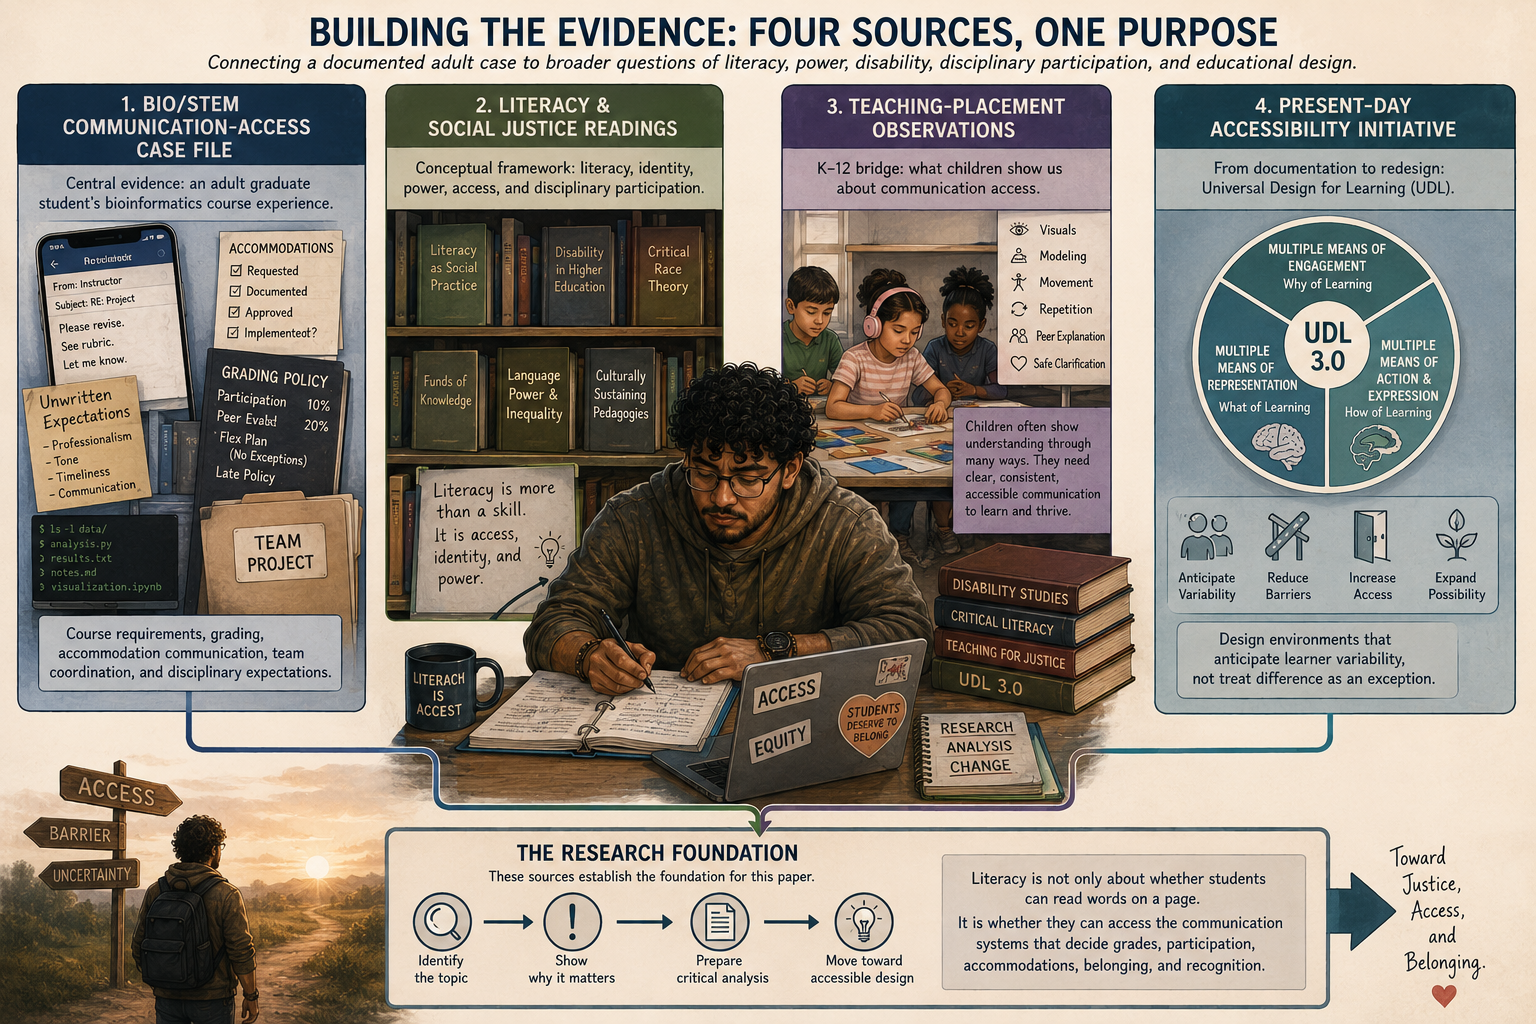
\includegraphics[
width=0.5\textwidth,
height=0.5\textheight,
keepaspectratio
]{images/building_the_evidence.png}
{\scriptsize\textit{Figure 3. How documented communication barriers, student effort, and institutional responses form a pattern of evidence pointing to systemic rather than individual failure.}\par}
\vspace{-1.5em}
\end{wrapfigure}

The analysis draws from four evidence sources. First, a \textit{BIO/STEM communication access case file} serves as the central site of inquiry, documenting barriers that emerged through unstated procedural expectations, grading language requiring interpretation beyond the written policy, health-related communication that increased burden during illness, accommodation procedures experienced as compliance checkpoints rather than access supports, collaborative project structures without explicit communication norms, and disciplinary terminology treated as self-evident rather than taught \citep{bioStemCaseFile2026}. Second, \textit{course readings in literacy and social justice} provide the conceptual framework, positioning literacy not as a technical skill but as a system of power that can recognize students as capable or mark them as deficient, invite participation or require students to earn it through hidden fluency \citep{knobel2007newliteracies,pricedennis2018digital}. Third, \textit{teaching placement observations} supply the school bridge; children typically demonstrate understanding through action, movement, peer collaboration, and embodied practice, yet they rarely possess the institutional language to name an access barrier as such \citep{teachingPlacementObservations2026}. Fourth, \textit{CAST UDL Guidelines 3.0} provides the present-day design framework, grounding recommendations in established accessibility scholarship \citep{cast2024udl}. Together, these sources establish the paper's central claim: communication access determines whether students are understood, supported, and allowed to belong, and designing it equitably is a matter of educational justice.

\newpage
%% ─────────────────────────────────────────────
\section*{Literacy as Communication Power: A Critical Analysis}
%% ─────────────────────────────────────────────

\begin{wrapfigure}{l}{0.5\textwidth}
\vspace{-3em}
\centering
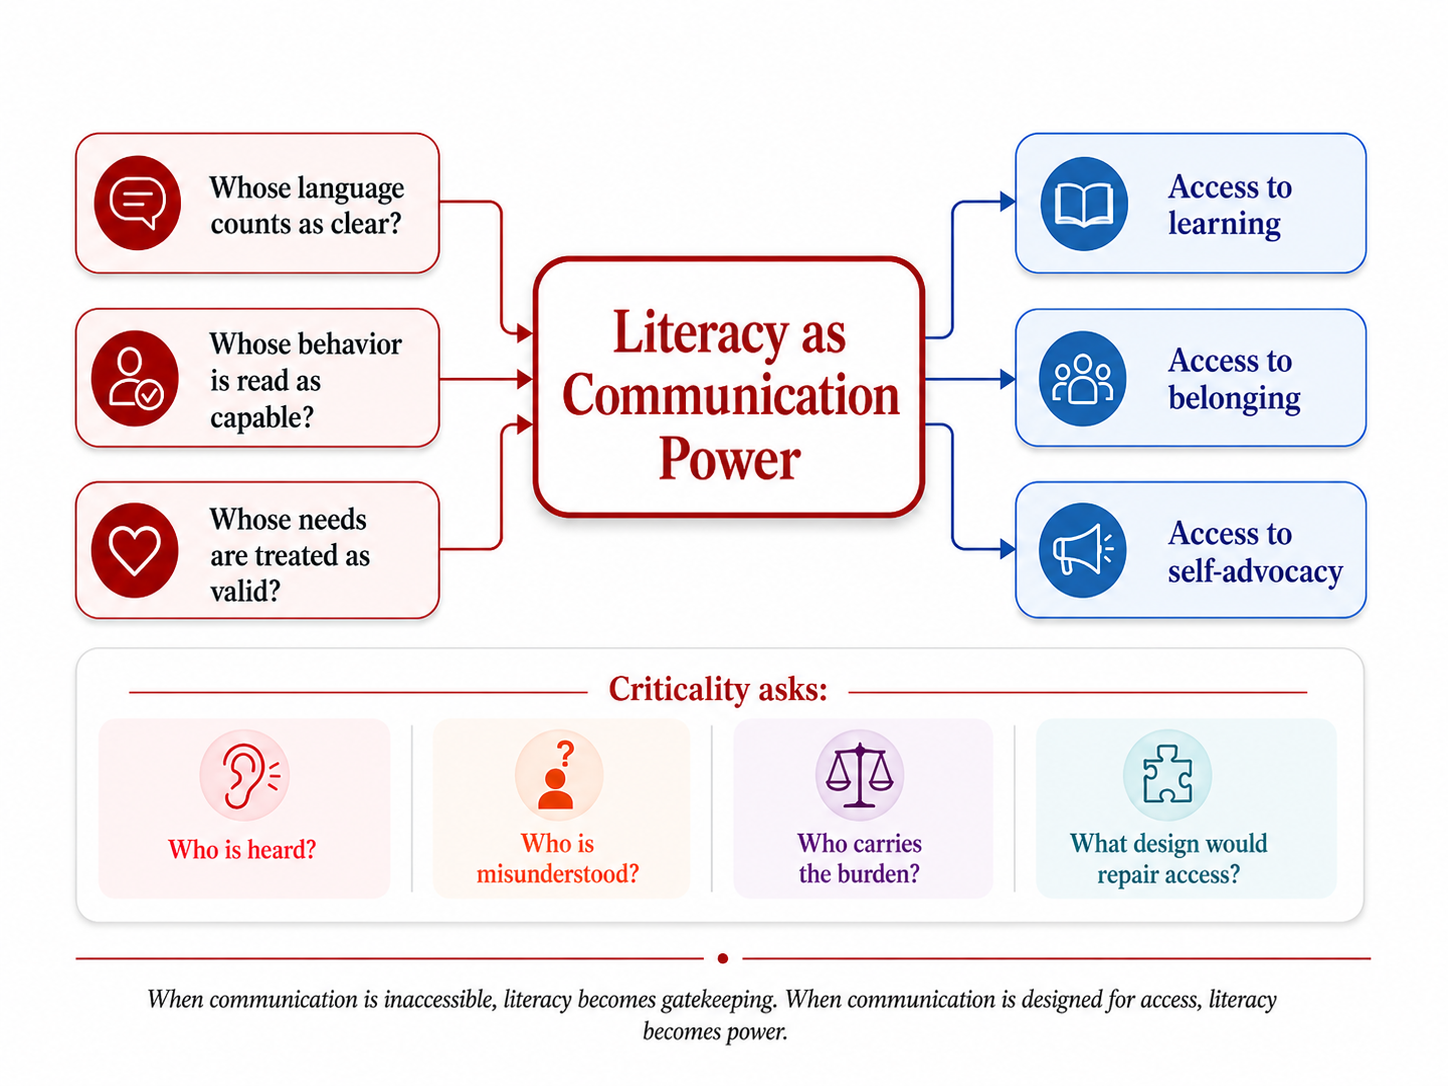
\includegraphics[
width=0.5\textwidth,
height=0.5\textheight,
keepaspectratio,
trim=1.2cm 0.4cm 1.2cm 0.3cm,
clip
]{images/literacy_as_communication_power.png}
{\scriptsize\textit{Figure 4. Literacy as power: how language recognition, behavioral interpretation, and access framing determine who is positioned as capable in the classroom.}\par}
\vspace{-2em}
\end{wrapfigure}

Communication access injustice is often invisible because it operates through language that sounds neutral. Terms like \textit{rigor}, \textit{professionalism}, \textit{participation}, \textit{reasonable accommodation}, and \textit{student responsibility} can appear fair while distributing burdens unevenly. A student without health barriers may experience an unclear requirement as a minor inconvenience, while a neurodivergent student may experience the same ambiguity as an executive function crisis, a chronically ill student may encounter it as one more demand layered over symptoms and disclosure fatigue, and a child may not experience it as ambiguity at all, only as shame, shutdown, or punishment. The words are the same; the weight is not.

\subsection*{Language, Authority, and Institutional Power}

A professor's communication carries institutional authority that students rarely meet as equals. Word choice, tone, and the channel through which expectations are delivered determine what counts as responsible, complete, professional, or valid; those determinations affect grades, standing, and access to support. The BIO/STEM evidence documents several patterns in which this authority operated as a barrier: procedural expectations communicated through unofficial or verbal channels became inaccessible for students whose neurocognitive profiles depend on stable written records; grading language that required interpretation beyond the written policy transformed assignments into policy-decoding tasks; health-related communication placed responsibility back on the student during moments of lowest capacity; accommodation language functioned as a compliance threshold rather than a design starting point; and team expectations communicated without explicit norms created an additional layer of burden over the academic work itself. What links these patterns is not individual carelessness but a shared structural assumption that students already know how to navigate the course itself, not just its content. For students who do not share that assumed literacy, the cost extends beyond confusion to executive function, health, identity, and future willingness to seek institutional support.

\subsection*{Terminology as Access or Exclusion}

Specialized language is legitimate and necessary in STEM; bioinformatics students must learn to read and write in the language of computational biology, including file formats, documentation conventions, code, and disciplinary communication practices. Specialized language becomes exclusionary, however, when it is treated as already known rather than explicitly taught. Terms such as \textit{Flex Plan}, \textit{DSO}, \textit{Ombuds}, \textit{peer evaluation}, \textit{formative feedback}, and \textit{professional communication} are not simple vocabulary; they are gatekeeping terms when students are expected to understand their procedural consequences without instruction. The goal is not to simplify STEM literacy but to make the path into it visible, so that students can learn the language of the field without simultaneously decoding hidden administrative rules under conditions of crisis.

\subsection*{Differential Burden and the School Stakes}

Different students bring fundamentally different forms of literacy to the same classroom. A graduate student may have advanced disciplinary knowledge and still lack the institutional literacy to interpret accommodation procedures or grading appeals; a neurodivergent student may show strong analytical capacity while requiring stable written expectations and explicit sequential structure; a chronically ill student may understand the material fully while needing communication systems that account for variable daily capacity; and a multilingual student may grasp a concept while being excluded by unexplained academic idioms embedded in the assignment itself. Children face even greater exposure because they typically lack both the language and the institutional standing to identify an access barrier as such; their response to inaccessible design tends to be behavioral, including shutdown, avoidance, repeated questioning, or apparent disengagement, and that behavior is itself subject to deficit interpretation. The BIO/STEM evidence functions here as a floor, not a ceiling. If a well-resourced adult can be meaningfully harmed by inaccessible course communication, the question is not whether children face comparable harm but how much deeper it runs when they cannot advocate for themselves.

\subsection*{Literacy as the Mediator of Justice}

Through the theoretical lens of the course readings, literacy is not pedagogically neutral \citep{knobel2007newliteracies,stornaiuolo2017writing}. It can recognize students as capable or position their needs as excessive; it can invite participation or require students to earn it by decoding rules that were never made explicit. \textit{It can support identity formation, or it can compel students to mask, over-document, and repeatedly justify their presence.} A classroom that admits only one mode of processing, remembering, or demonstrating knowledge is not rigorous in any meaningful sense; it is selective, rewarding students who already hold the expected literacy profile and penalizing students whose literacies appear in other forms. The corrective is not lower standards but clearer ones: expectations made visible, disciplinary language explicitly taught, feedback structured accessibly, and accommodations treated as the beginning of design rather than the boundary of obligation.

%% ─────────────────────────────────────────────
\section*{UDL, Teaching Practice, and Student Vulnerability}
%% ─────────────────────────────────────────────

\begin{wrapfigure}{l}{0.5\textwidth}
\vspace{-2em}
\centering
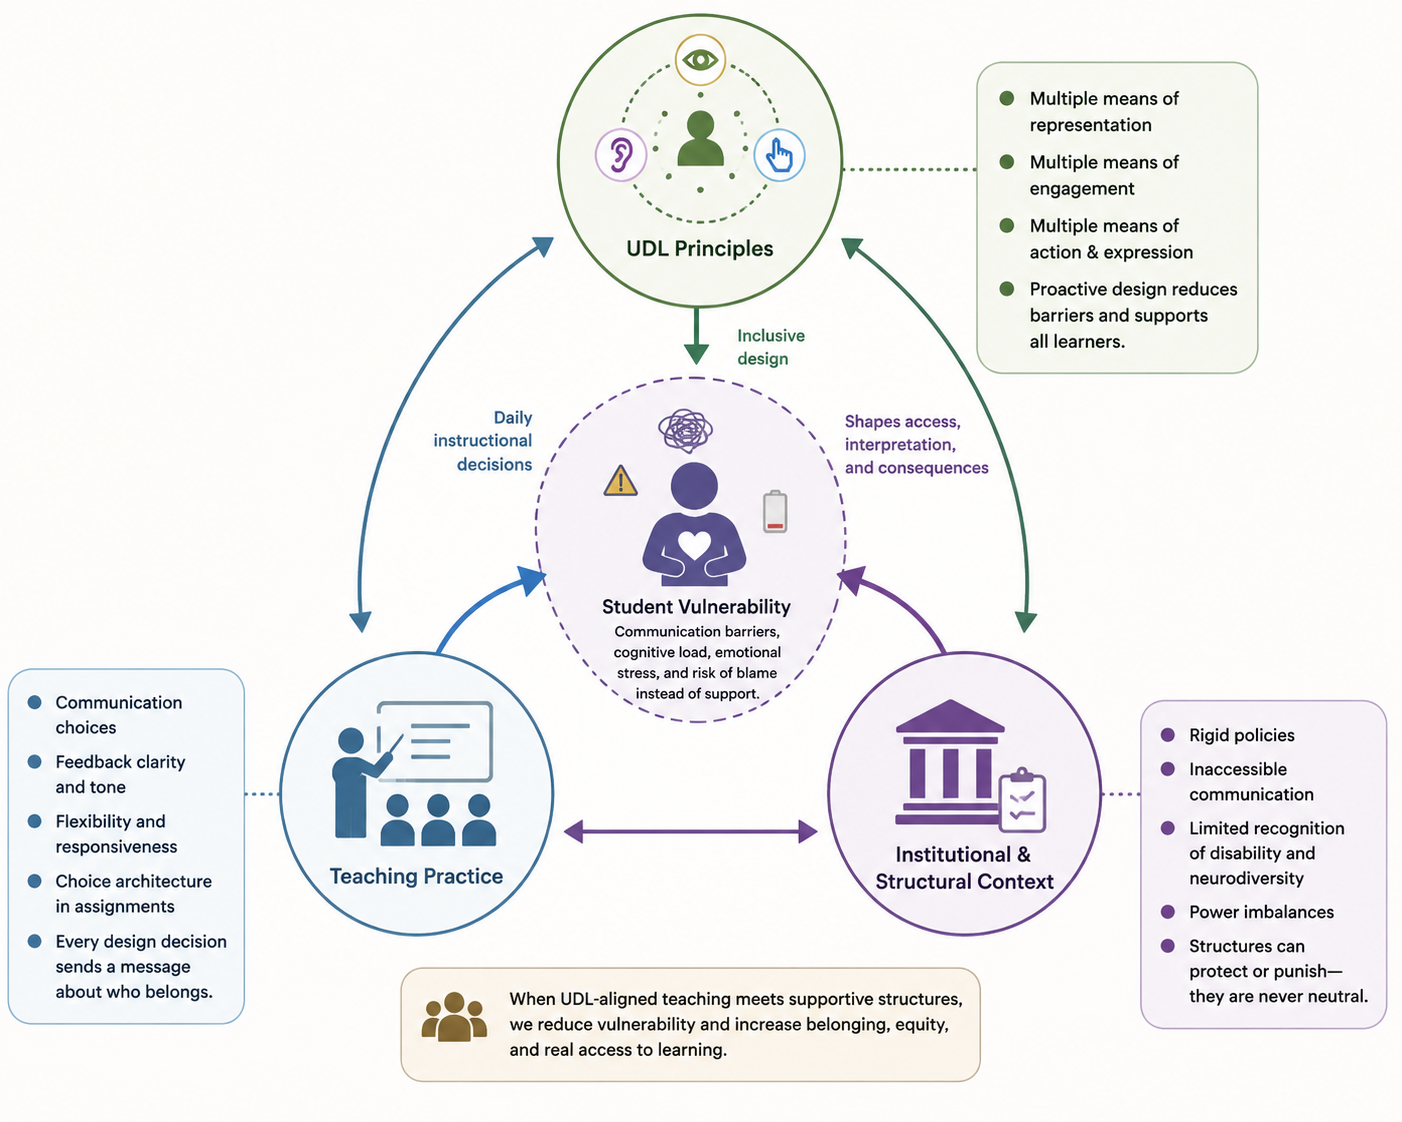
\includegraphics[
width=0.5\textwidth,
height=0.5\textheight,
keepaspectratio
]{images/connecting_issues_to_the_present.png}
{\scriptsize\textit{Figure 5. How UDL, institutional structures, and communication design together shape and reduce student vulnerability.}\par}
\vspace{-1em}
\end{wrapfigure}

Universal Design for Learning, particularly the \textit{CAST UDL Guidelines 3.0}, directly addresses the conditions documented in this paper \citep{cast2024udl}. UDL reframes the question from \textit{how do we help students after they struggle?} to \textit{how do we design learning environments so access is embedded before struggle occurs?} The Guidelines name learner agency as the goal: learners who are purposeful and reflective, resourceful and authentic, and strategic and action-oriented; that goal is structurally incompatible with communication systems that require students to survive the course design before they can engage with its content. The primary audience for UDL is educators and curriculum designers, those who decide whether instructions are spoken or written, whether technical language is modeled or assumed, and whether accommodations are treated as access supports or compliance minimums. A neurodivergent or chronically ill student should not be expected to master institutional navigation, disability services, and professor communication management simply to complete a semester; children are even less equipped for that role.

UDL operationalizes access through four commitments. \textit{Multiple means of representation} ensure that important information is not dependent on any single channel; it is available in stable written form, modeled visually, defined in plain language alongside technical vocabulary, and findable after the synchronous session ends. \textit{Language and symbolic accessibility} require that disciplinary terms, institutional processes, and grading criteria be explicitly defined, illustrated through examples, and revisited across the course rather than front-loaded once. \textit{Multiple means of action and expression} recognize that students demonstrate knowledge through writing, code, design, oral explanation, revision, and peer teaching, not only through one approved format. \textit{Belonging, emotional safety, and learner agency} acknowledge that a student who feels threatened or penalized for seeking clarification cannot access learning even when content is technically present \citep{cast2024udl}. UDL is not immune to co-optation; a course may claim to value learner variability while retaining single-mode instructions, ambiguous grading policies, and accommodation procedures that communicate compliance rather than care. \textit{Access is a design decision repeated every class period}, not a philosophical commitment made once at the syllabus level.

My teaching placement observations clarify what is at stake in school settings. Children regularly show understanding through movement, building, drawing, peer explanation, and physical experimentation. When a student asks the same question repeatedly, avoids starting, or copies a peer's process, the barrier may not be comprehension; it may be that the task structure, the language of the directions, or the absence of a visual model has made the entry point inaccessible. Treating that behavior as evidence of low ability, rather than as diagnostic information about the learning environment, is the moment where a literacy system stops being educational and starts being exclusionary \citep{teachingPlacementObservations2026}.

%% ─────────────────────────────────────────────
\section*{Connecting to the Present: CAST UDL in Practice}
%% ─────────────────────────────────────────────

\begin{wrapfigure}{r}{0.46\textwidth}
\vspace{-2em}
\centering
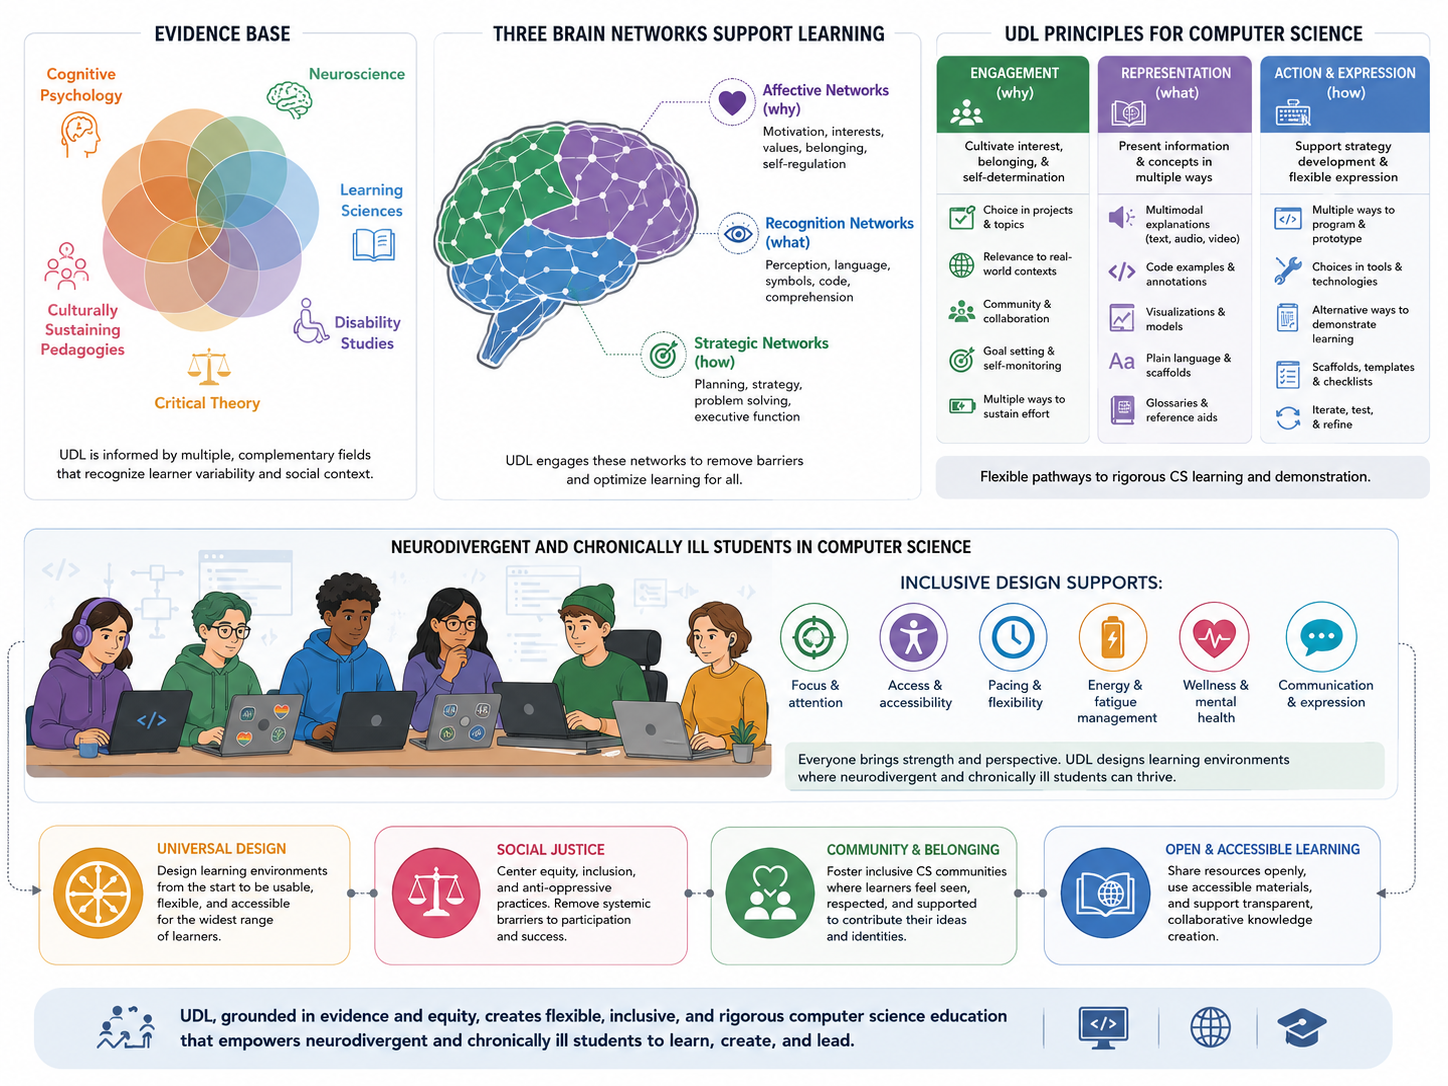
\includegraphics[width=0.46\textwidth,height=0.46\textheight,keepaspectratio]{images/UDL_for_computer_science.png}
{\scriptsize\textit{Figure 7. CAST UDL Guidelines 3.0 as the present-day initiative connecting communication access, learner variability, and inclusive instructional design in computer science contexts.}\par}
\vspace{-1em}
\end{wrapfigure}

The present-day initiative examined here is the \textit{CAST Universal Design for Learning Guidelines 3.0}, a publicly accessible framework that translates research on learner variability into design guidance for educators, curriculum designers, instructional leaders, and institutional support systems \citep{cast2024udl}. I also treat the public communication surrounding UDL as part of the initiative because the way a framework is communicated determines who can understand it, use it, and invoke it when institutions fail to practice it. The visual syntheses in this section are original supporting figures for this journal; they represent how UDL principles circulate across teacher-facing, student-facing, and broader public communication without reproducing any specific organizational post.

\subsection*{Target Audience and Literacy Levels}

CAST's primary audience is \textit{educators, curriculum designers, administrators, and instructional coaches}, not students or families. The Guidelines are written in specialist educational language, presuppose familiarity with terms like \textit{executive function}, \textit{metacognition}, \textit{self-regulation}, and \textit{affective networks}, and embed research citations throughout; that register is appropriate for the primary audience but also means that the students and families most affected by the practices UDL is designed to change are not necessarily positioned as direct readers of the framework. This is the literacy tension at the center of this assignment: a framework can be designed for justice while still requiring translation before it becomes usable by the communities most affected by injustice.

\begin{wrapfigure}{l}{0.46\textwidth}
\vspace{-1em}
\centering
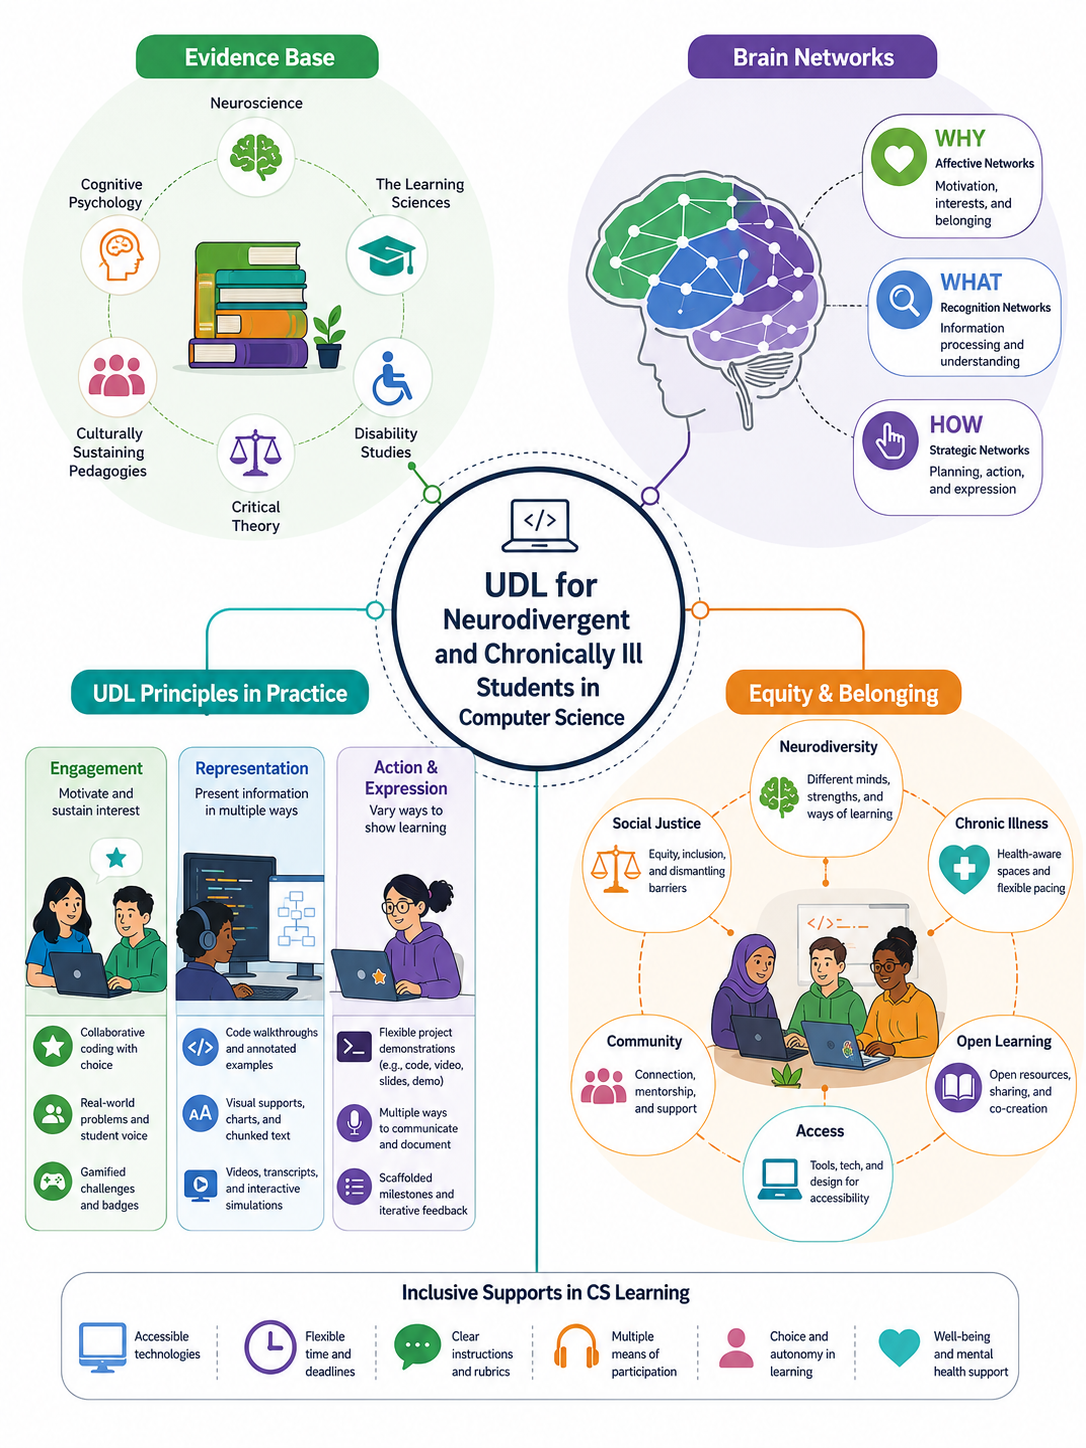
\includegraphics[width=0.46\textwidth,height=0.46\textheight,keepaspectratio]{images/UDL_for_chronically_ill_and_neurodivergents.png}
{\scriptsize\textit{Figure 8. Original visual synthesis showing how UDL principles support neurodivergent and chronically ill students through engagement, representation, flexible expression, belonging, and pacing.}\par}
\vspace{-1em}
\end{wrapfigure}

Digital literacy research from the course helps explain why the same initiative may need multiple registers. Website language can serve policy and professional audiences, while visual summaries, student-facing guides, and community dialogue create wider access. This reflects the course readings on new literacies and digital participation, which emphasize that literacy practices are social, multimodal, identity-linked, and shaped by the communities in which they circulate \citep{knobel2007newliteracies,pricedennis2018digital,stornaiuolo2017writing}. In this sense, UDL is not only a content framework; it is also a communication challenge. The framework must be readable across professional, classroom, family, and student audiences if it is going to protect the students it names.

\subsection*{Strategies for Inclusive Communication}

\begin{wrapfigure}{r}{0.46\textwidth}
\vspace{-1em}
\centering
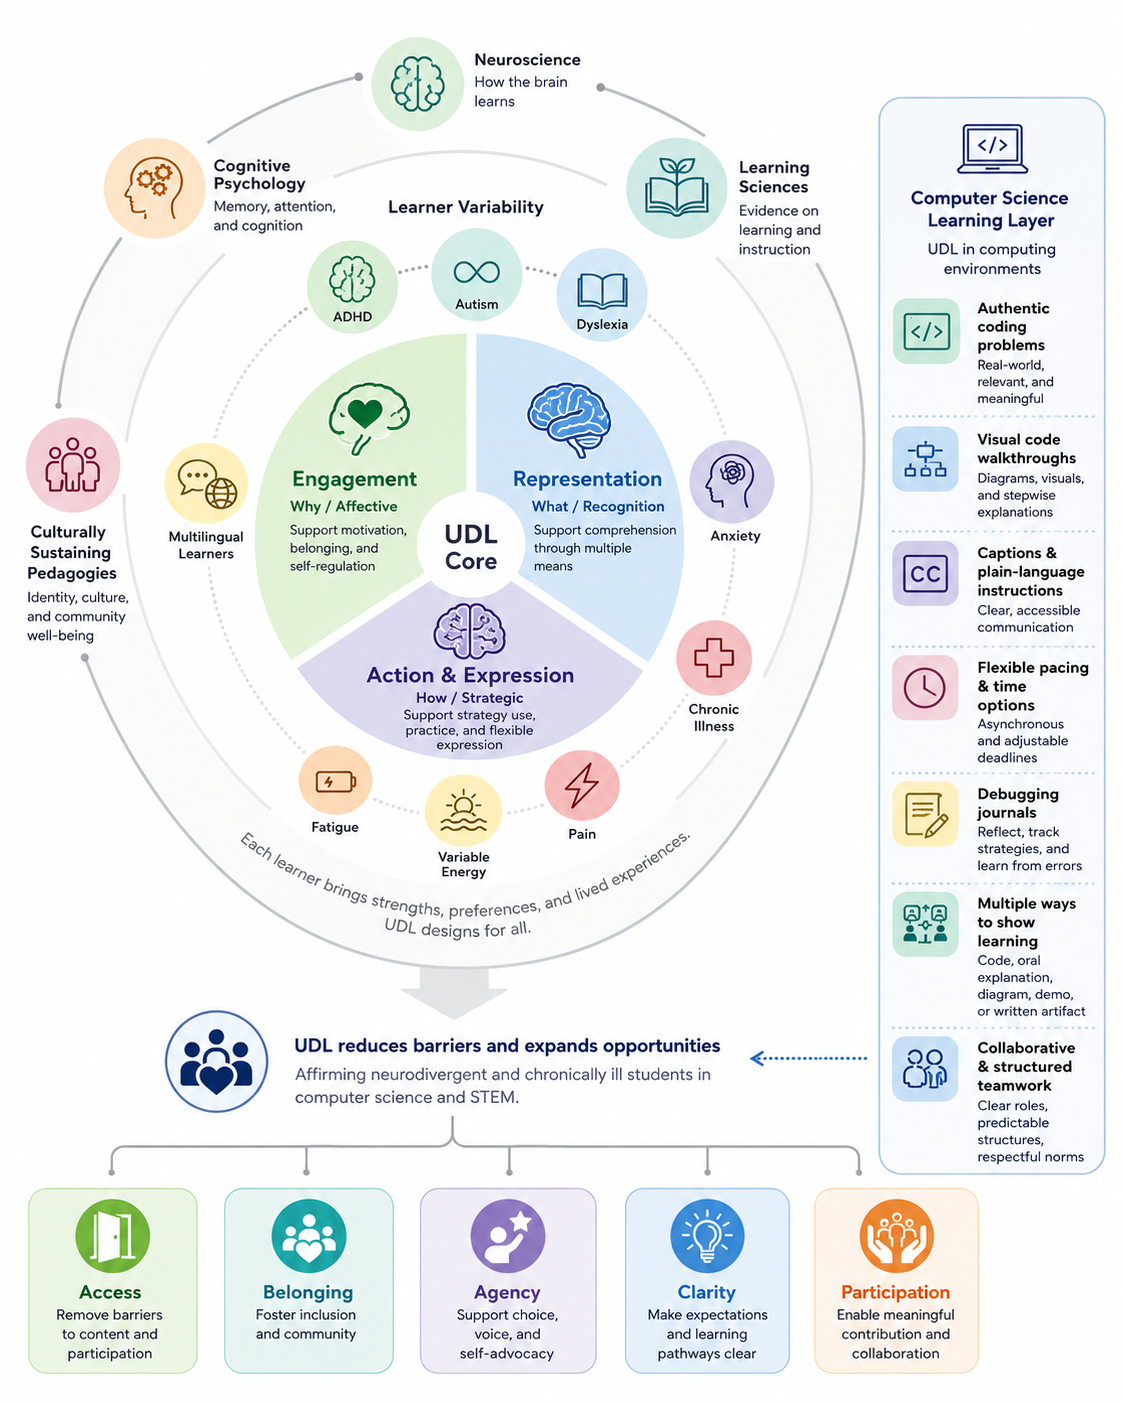
\includegraphics[width=0.46\textwidth,height=0.46\textheight,keepaspectratio]{images/UDL_CAST_social_media.png}
{\scriptsize\textit{Figure 9. Original visual synthesis showing how UDL evidence, brain network research, open access design, social justice, and community practice work together to reduce barriers for neurodivergent and chronically ill students.}\par}
\vspace{-2em}
\end{wrapfigure}

CAST's communication employs several strategies that align directly with the accessibility principles this paper advocates for classrooms. The Guidelines website offers \textit{multiple means of representation}; each checkpoint is organized through labels, short descriptions, and expandable rationales with linked research. The framework's visual organization, including color-coded columns, headings, and icons, makes the architecture of UDL legible before a visitor reads every sentence, modeling the same multimodal clarity it recommends for teachers \citep{cast2024udl}. Public and community-facing communication can further distribute access points across literacy levels through infographics, brief practitioner stories, and shared hashtag communities; this follows the same logic Stornaiuolo and Thomas (2017) describe in youth civic digital literacy, where communication that reaches across audiences requires deliberately designed, multiple entry points \citep{stornaiuolo2017writing}. The Common Sense Digital Citizenship curriculum, an EDU498 Module 3 resource, uses a comparable layered access model in which teacher guides, student-facing materials, and family resources are written at distinctly different registers, each self-sufficient yet linked \citep{commonsense2023digital}; that model is directly applicable to syllabi, assignment instructions, and accommodation pathways in higher education.

\subsection*{Communication Barriers Caused by Literacy Challenges}

Despite its accessible design ambitions, CAST's communication faces three significant barriers. First, \textit{institutional gatekeeping}: the UDL framework typically reaches educators through professional development and graduate training rather than directly reaching students or families; a neurodivergent student navigating an inaccessible course rarely has access to the policy vocabulary that would allow them to name what is happening, and they do not automatically receive a usable UDL translation alongside their syllabus. Second, \textit{implementation gap}: CAST's communication is aspirational and descriptive, not enforceable; a course can cite UDL on its syllabus and still retain single-mode instructions, oral-only policy updates, and accommodation language used as a compliance threshold. Third, \textit{disproportionate reach}: the National Center for Learning Disabilities documents that students of color, particularly Black and Hispanic students, are simultaneously overidentified for disability labels that restrict access and underidentified for services that provide support \citep{ncld2020disproportionality}; CAST's framework, however carefully designed, does not reach these students equally when the institutions implementing it carry structural inequities that UDL alone cannot correct. These barriers do not disqualify UDL as a framework; they clarify what frameworks require in order to function as justice instruments: institutional accountability, student-facing communication, and a genuine interrogation of who the default learner in any given course has been assumed to be.

%% ─────────────────────────────────────────────
\section*{Recommendations: Designing Access Before Harm}
%% ─────────────────────────────────────────────

\begin{wrapfigure}{r}{0.5\textwidth}
\vspace{-4em}
\centering
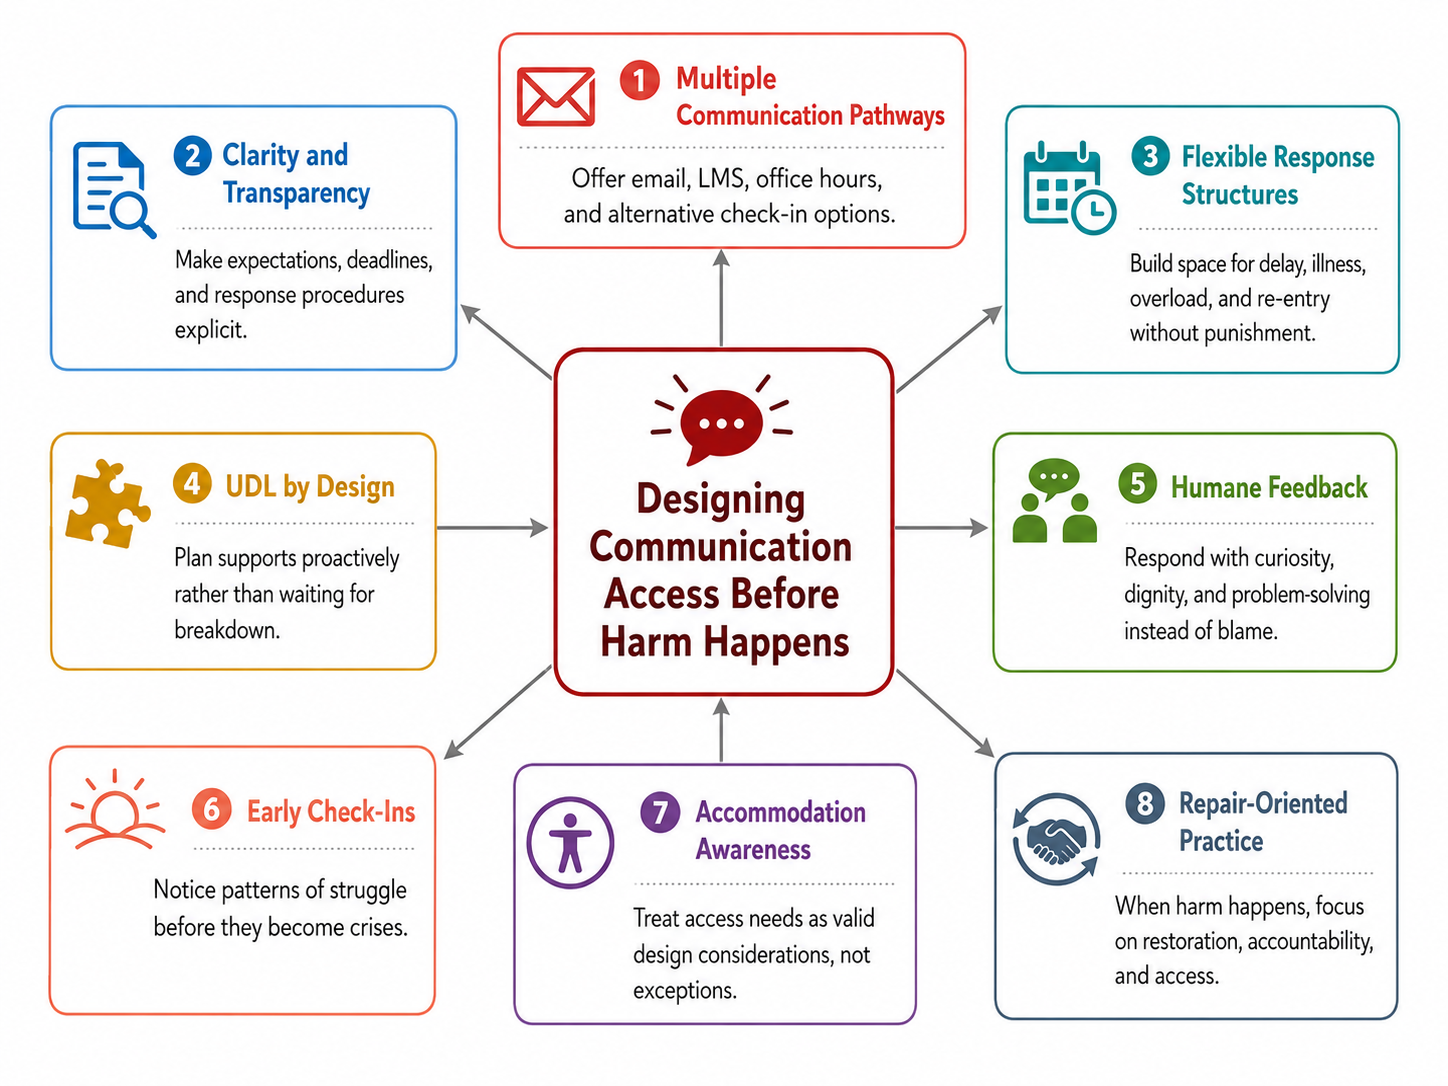
\includegraphics[
width=0.5\textwidth,
height=0.5\textheight,
keepaspectratio
]{images/designing_communication_access.png}
{\scriptsize\textit{Figure 10. Core recommendations for designing communication access before harm occurs.}\par}
\vspace{-3em}
\end{wrapfigure}

The following recommendations are not concessions to lower standards; they are preconditions for those standards to be meaningfully applied. \textit{Stable, centralized written expectations} require that any expectation affecting a grade, submission, participation score, or peer evaluation be available in writing, findable after class, and updated in writing when it changes; students who depend on written records, whether by neurocognitive profile, language background, or health condition, should not be required to reconstruct official requirements from memory. \textit{Accommodations as design starting points} means that access should not be gated behind formal accommodation letters; reducing unnecessary memory demands, clarifying implied expectations, posting changes in writing, and building flexible response structures into course design serve all students while disproportionately protecting those who need them most.

\textit{Explicit instruction in disciplinary literacy} requires that scientific language, technical documentation conventions, institutional terminology, and grading criteria be taught, modeled, defined, and revisited rather than assumed; students learning bioinformatics are simultaneously learning how to communicate in the discipline, and that process requires scaffolding. \textit{Structured team communication norms} mean that collaborative projects require explicit written agreements covering roles, tools, decision-making processes, protocols for illness or missed contributions, peer-evaluation criteria, and private escalation pathways; leaving team communication entirely informal does not simulate professional practice but amplifies access inequality. \textit{Multiple modes of demonstration} means that spoken directions should be paired with written equivalents, technical vocabulary with plain-language glosses, feedback with examples, and courses should create legitimate pathways for students to show understanding through writing, code, design, oral explanation, revision, and collaborative process, not only through a single output format.

The underlying shift is from accommodation as exception to communication access as standard practice. The diagnostic question should not be \textit{what is wrong with this student?} but \textit{what does this course require students to decode, remember, and navigate before they are allowed to demonstrate what they know?} That question holds students accountable while locating educator responsibility where it belongs: in the design of the learning environment.

%% ─────────────────────────────────────────────
\section*{From Pain to Protection: A Critical Reflection}
%% ─────────────────────────────────────────────

This assignment required me to think about literacy as something larger than reading and writing, as the set of systems that determine whether a person is understood, included, and allowed to participate. That reframing changed how I interpreted the BIO/STEM evidence: what could appear to be isolated miscommunication resolves, through a literacy and social justice lens, into a pattern, the consistent displacement of access burden onto the student least equipped to carry it during moments of highest demand. I was an adult graduate student with technical expertise, documentation practices, an advisor, and the institutional language to name a design problem as a design problem; even with those resources, the communication environment affected my health, my confidence in the institution, and my capacity to participate fully. That is not a complaint about difficulty, which belongs in graduate education; it is an account of a system that added harm where harm was not necessary.

Children cannot make that distinction. They can only live it. When a student shuts down during a task they otherwise understand, the behavior is communication, not evidence of low capacity but diagnostic information about the learning environment. My teaching placement has reinforced that the difference between those two interpretations, capacity problem or design problem, determines what a teacher does next and what the student internalizes as a result. This reflection also connects to my research in equity and algorithmic systems; a classroom can misclassify a student the same way an algorithm can misclassify a patient, by using inputs that appear objective while encoding structural exclusions into the definition of normal \citep{ncld2020disproportionality}. Whether the system is a diagnostic model or a course grading structure, the question is the same: \textit{who is being misread, and what would it take to redesign the system so they are seen more accurately?}

Universal Design for Learning provides a framework, but frameworks are only as powerful as the daily decisions they shape \citep{cast2024udl}. Accessibility is a practice, repeated in how directions are written, how vocabulary is taught, how feedback is structured, how changes are communicated, and how behavior is interpreted; every one of those moments is a choice about who the classroom is designed for. I am writing from my own experience because it is the evidence I can document, but the argument is not for myself; it is for the students who come after me, particularly the younger, quieter, sicker, more frightened, less resourced, and less institutionally fluent. Communication access is the doorway into learning. When that doorway is designed narrowly, it does not select for the most capable students; it selects for the students who already know how to open it. A just classroom widens that doorway; it does not lower the destination but makes the path visible.

\newpage
\bibliographystyle{apalike}
\bibliography{references}
\end{document}
